\subsection{ 激活函数}

激活函数是深度学习的灵魂，它为神经网络注入了非线性，让模型能够捕捉复杂的特征。比如，ReLU函数的简单性和效率，使其成为深度学习的“主力军”。



激活函数是神经网络的关键组件，用于引入非线性能力，使网络能够表达复杂的模式。常见的激活函数包括：

Sigmoid 函数：用于将输出限制在 $[0, 1]$ 范围。
ReLU 函数：高效且常用，解决了梯度消失问题。
Tanh 函数：扩展了 Sigmoid 的输出范围至 $[-1, 1]$。


{\bf 非线性表达需要激活函数}

任何线性函数的线性组合仍然是线性的。
没有激活函数，神经网络就是线性函数，不能解决任何非线性问题。


{\bf  通用近似定理(universal approximation theorem) (Hornik et al., 1989; Cybenko, 1989) }

对于具有线性输出层和至少一个使用 “挤压”性质的激活函数的隐藏层组成的前馈神经网络，只要其隐藏层神经元的数量足够，可以以任意精度近似任一个定义在实数空间中的有界闭集函数。

一个两层的神经网络可以模拟任何函数。



神经网络能逼近任何函数：分段是关键。任何函数，可以用“分段”线性函数来逼近

激活函数，让神经网络具备“分段”表达能力。

\begin{figure}[htbp]
\centering
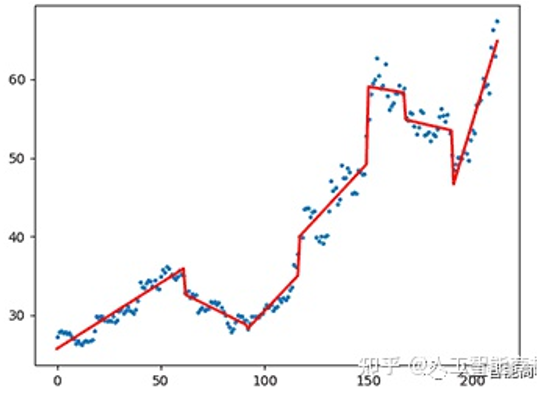
\includegraphics[width=0.69\textwidth]{figs/分段线性逼近.png}
\caption{分段线性函数的逼近}
\label{分段线性逼近}
\end{figure}


{\bf 激活函数的分段功能} 

激活函数为神经网络提供“分段”能力的来源。
激活函数 activation =“打开”+ “截断”能力
Relu激活函数
	输入~$𝑥<0$ 时，输出~$𝑦=0$ ，实现截断(关闭)功能
	输入~$𝑥>0$ 时，输出~$𝑦=𝑥$，实现导通(打开)功能。
激活函数的“分段”能力，把线性函数，组合成折线函数（分段函数），可以让神经网络逼近任何函数。

{\bf 神经网络近似任意函数的示例}

最简单的神经网络：最后一层是Sigmoid函数：
一个线性函数经过Sigmoid扭曲为一条“S型”曲线。

只要有足够多的分段函数，并仔细调整它们的权重，就能近似任意的函数。

思想类似于傅里叶级数定理：复杂周期运动 = 多个周期运动之和
      非周期运动 = 无穷个周期运动之和



%\begin{figure}[htbp]
%\centering
%begin{subfigure}{0.6\linewidth}
%\centering
%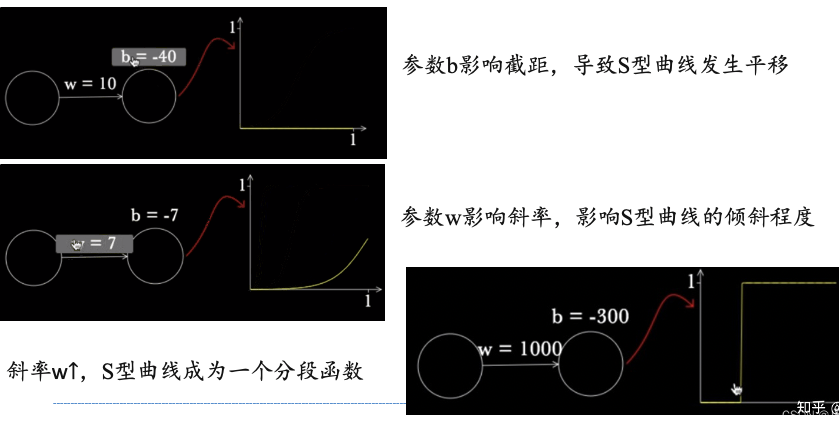
\includegraphics[width=1\linewidth]{figs/神经网络近似任意函数.png}
%\caption{神经网络近似任意函数}
%\label{神经网络近似任意函数}
%\end{subfigure}
%
%begin{subfigure}{0.6\linewidth}
%\centering
%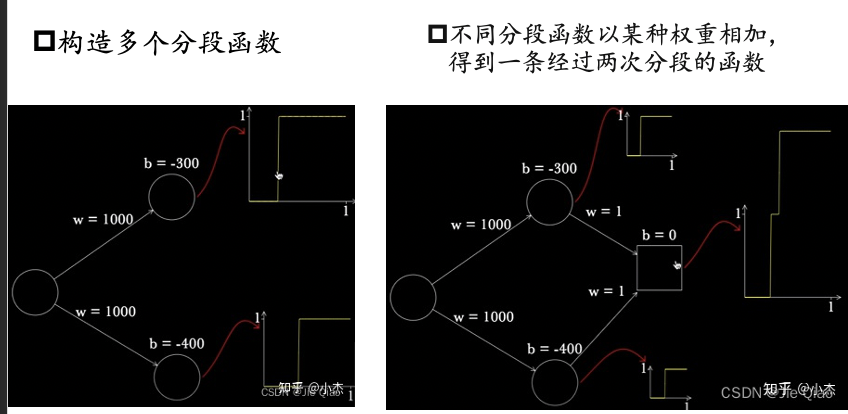
\includegraphics[width=1\linewidth]{figs/神经网络近似任意函数2.png}
%\caption{神经网络近似任意函数2}
%\label{神经网络近似任意函数2}
%\end{subfigure}
%\caption{神经网络近似任意函数}
%\label{神经网络近似任意函数}
%\end{figure}



{\bf 万能近似原理的一维与~$n$维情形}


\begin{figure}[htbp]
\centering
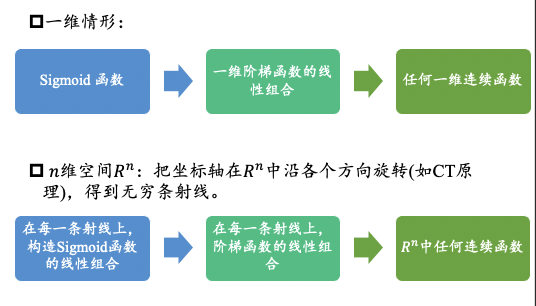
\includegraphics[width=0.69\textwidth]{figs/万能近似定理.png}
\caption{万能近似定理}
\label{万能近似定理}
\end{figure}


截断能力最强的是阶跃函数和ReLu函数，其它激活函数：“软化”版（折线变曲或变缓）
梯度下降法需要求解相邻层的梯度，这要求网络中处处可导，故激活函数需满足可导性。
M-P模型中使用step函数作为激活函数，只能输出0或1，不连续不可导。
后续提出可导函数sigmoid作为激活函数---梯度饱和问题
发展出ReLU函数及其变形激活函数


\begin{figure}[htbp]
\centering
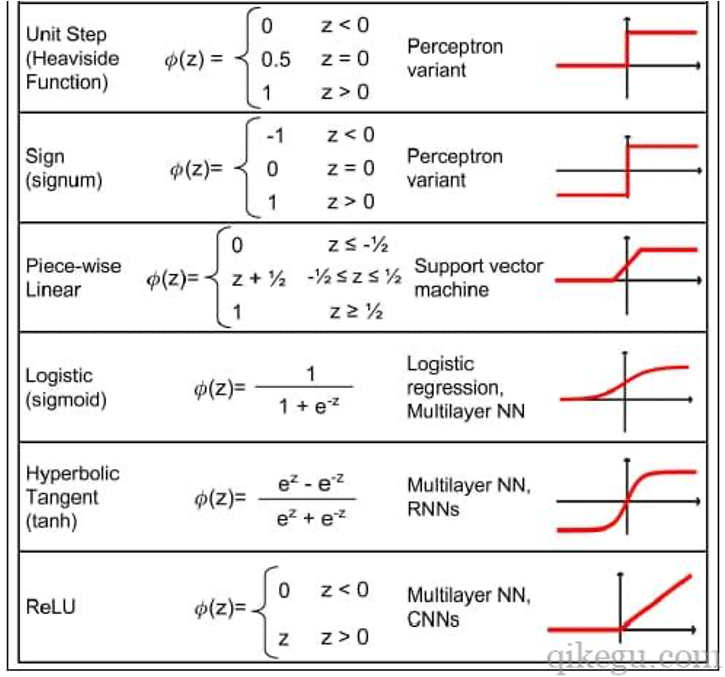
\includegraphics[width=0.69\textwidth]{figs/激活函数.png}
\caption{激活函数}
\label{激活函数}
\end{figure}

{\bf  Unit Step Function (Heaviside Function)}

{\bf  Unit Step Function (Heaviside Function)}

{\bf  Piece-wise Linear }


{\bf  Logisitic (sigmoid)}

劣势：
输入趋近无穷时会导致梯度趋近于零：引起梯度弥散
所有输出值均为正值，不以零为中心：影响神经网络收敛速度

如何改进---Tanh函数：
以零为中心的对称函数，收敛速度快
仍然无法解决梯度弥散问题

梦魇： “梯度消失”现象严重。
梯度指数衰减后，在反向传播时，底层基本上接受不到有效的训练信号。
如，幅度为1的信号，在反向传播梯度时，每传递一层，梯度衰减为原来的0.25。




新函数的应用：
在DNN的发展中，ReLU、maxout等传输函数代替了 Sigmoid，解决了梯度消失问题。


融合使用的试验：e.g. Sigmoid系的Acrtan函数和ReLU函数的融合


{\bf Hyperbolic Tangent(tanh)  }

{\bf  ReLU 函数 (Rectified Linear Unit，ReLU)}

ReLU函数
分散、稀疏，避免了Sigmoid系函数的饱和情况
有利于梯度下降和反向传播算法，避免梯度爆炸和梯度消失
小于零的部分均为零：硬饱和性，均值偏移

1. 计算速度快
2. 生物上的原因
3. 解决梯度下降问题


\begin{figure}[htbp]
\centering
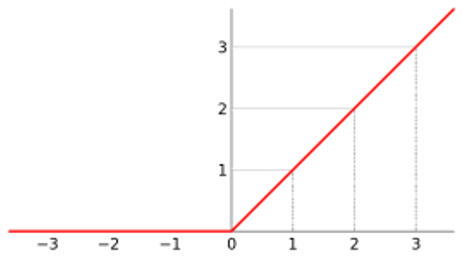
\includegraphics[width=0.69\textwidth]{figs/ReLU.png}
\caption{ReLU}
\label{ReLU}
\end{figure}


\begin{figure}[htbp]
\centering
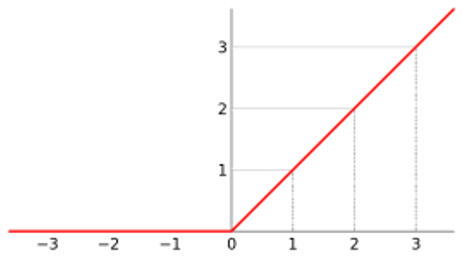
\includegraphics[width=0.69\textwidth]{figs/ReLU.png}
\caption{ReLU}
\label{ReLU}
\end{figure}


%\begin{figure}[htbp]
%\centering
%begin{subfigure}{0.6\linewidth}
%\centering
%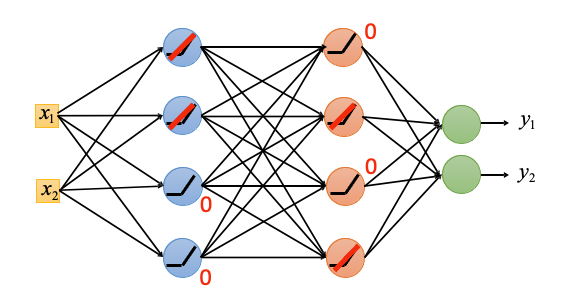
\includegraphics[width=1\linewidth]{figs/ReLU-network.png}
%%\caption{}
%\label{ReLU-network}
%\end{subfigure}

%begin{subfigure}{0.6\linewidth}
%\centering
%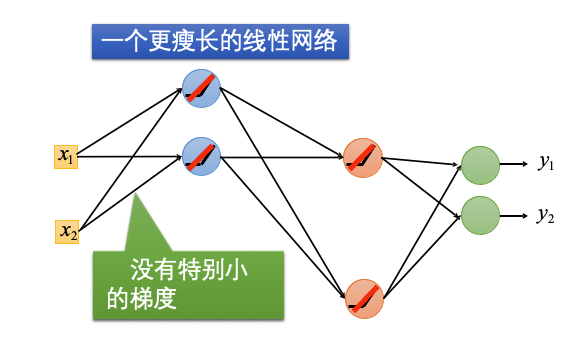
\includegraphics[width=1\linewidth]{figs/ReLU-network2.png}
%%\caption{}
%\label{ReLU-network2}
%\end{subfigure}
%\caption{神经网络近似任意函数}
%\label{神经网络近似任意函数}
%\end{figure}
%
%\begin{figure}[htbp]
%\centering
%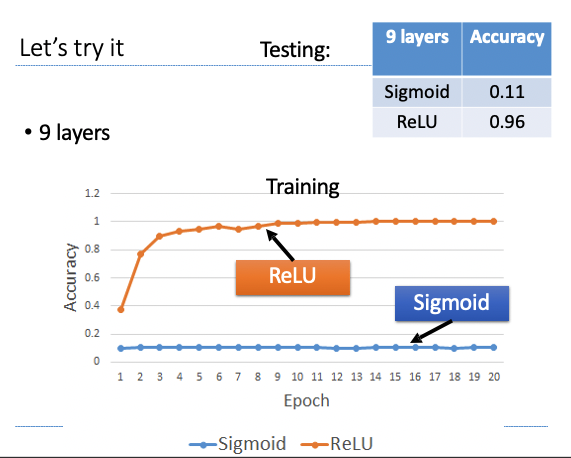
\includegraphics[width=0.69\textwidth]{figs/experiement.png}
%\caption{ReLU 函数与Sigmoid 函数对比}
%\label{experiement}
%\end{figure}
%

{\bf  Arctan}

Arctan函数
基本性质类似Sigmoid函数
输出范围在 (- π / 2 , π / 2 )
比Sigmoid函数和Tanh函数图像更为和缓，饱和区间较大
导数趋于零的速度更慢，导数计算更加昂贵，但缓解了梯度消失问题

\begin{figure}[htbp]
\centering
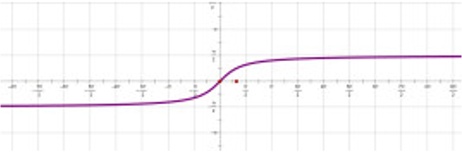
\includegraphics[width=0.69\textwidth]{figs/arctan.png}
\caption{arctan}
\label{arctan}
\end{figure}


{\bf AcrReLU函数}

~$x>0$的部分采用ReLU函数
~$x\le0$的部分采用Acrtan函数


实验效果：
初始的累积误差小，具有较快的收敛速度。
有效缓解梯度消失问题
缓解ReLU负轴部分的硬饱和性
AUC值更大，泛化性能更优
但计算消耗较昂贵，时间较久
\begin{figure}[htbp]
\centering
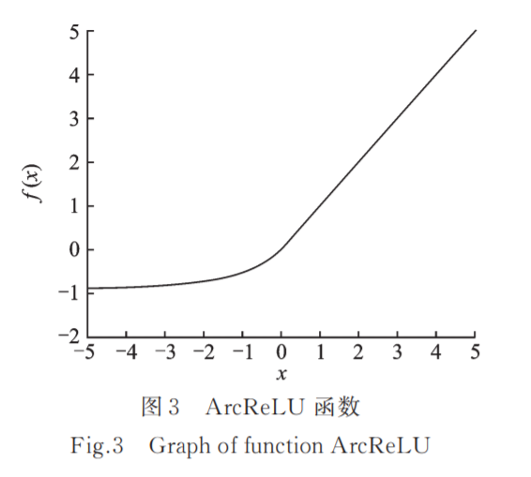
\includegraphics[width=0.69\textwidth]{figs/arcReLU.png}
\caption{arcReLU}
\label{arcReLU}
\end{figure}


深度学习的关键在于非线性变换，而激活函数正是引入非线性的关键部分。

常见的激活函数有：

Sigmoid：适用于概率输出，但易于梯度消失。
Tanh：改进了Sigmoid，但仍然存在梯度消失问题。
ReLU（Rectified Linear Unit）：计算高效，解决了梯度消失问题，是目前最常用的激活函数。


常用 ReLU（Rectified Linear Unit）作为非线性激活函数，定义为：
$$
f(x)=max(0,x)$$

ReLU 引入了非线性能力，使网络能够拟合复杂的模式。


